\documentclass[11pt]{article}
\usepackage[textwidth=18.0cm, textheight=23.0cm, top=2.0cm]{geometry}
\usepackage{pst-all}
\usepackage{amssymb}
\usepackage{tikz}
\usepackage{underscore}\begin{document}
\pagestyle{empty}


ClassName: \underline{\textbf{Class_08.2bp-16}}
\par
BinSize: \underline{\textbf{100 × 100}}
\par
ReduceSize: \underline{\textbf{100 × 100}}
\par
TypeNum: \underline{\textbf{39}}
\par
Num: \underline{\textbf{40}}
\par
OutS: \underline{\textbf{110000}}
\par
InS: \underline{\textbf{88625}}
\par
Rate: \underline{\textbf{0.806}}
\par
UB: \underline{\textbf{11}}
\par
LB0: \underline{\textbf{11}}
\par
LB: \underline{\textbf{11}}
\par
LBWithCut: \underline{\textbf{11}}
\par
NodeCut: \underline{\textbf{0}}
\par
ExtendedNodeCnt: \underline{\textbf{1}}
\par
GenNodeCnt: \underline{\textbf{1}}
\par
PrimalNode: \underline{\textbf{0}}
\par
ColumnCount: \underline{\textbf{11}}
\par
TotalCutCount: \underline{\textbf{0}}
\par
RootCutCount: \underline{\textbf{0}}
\par
LPSolverCnt: \underline{\textbf{1}}
\par
PricingSolverCnt: \underline{\textbf{0}}
\par
BranchAndBoundNum: \underline{\textbf{1}}
\par
isOpt: \underline{\textbf{true}}
\par
TimeOnPrimal: \underline{\textbf{0.000 s}}
\par
TimeOnPricing: \underline{\textbf{0.000 s}}
\par
TimeOnRmp: \underline{\textbf{0.063 s}}
\par
TotalTime: \underline{\textbf{0.125 s}}
\par
\newpage


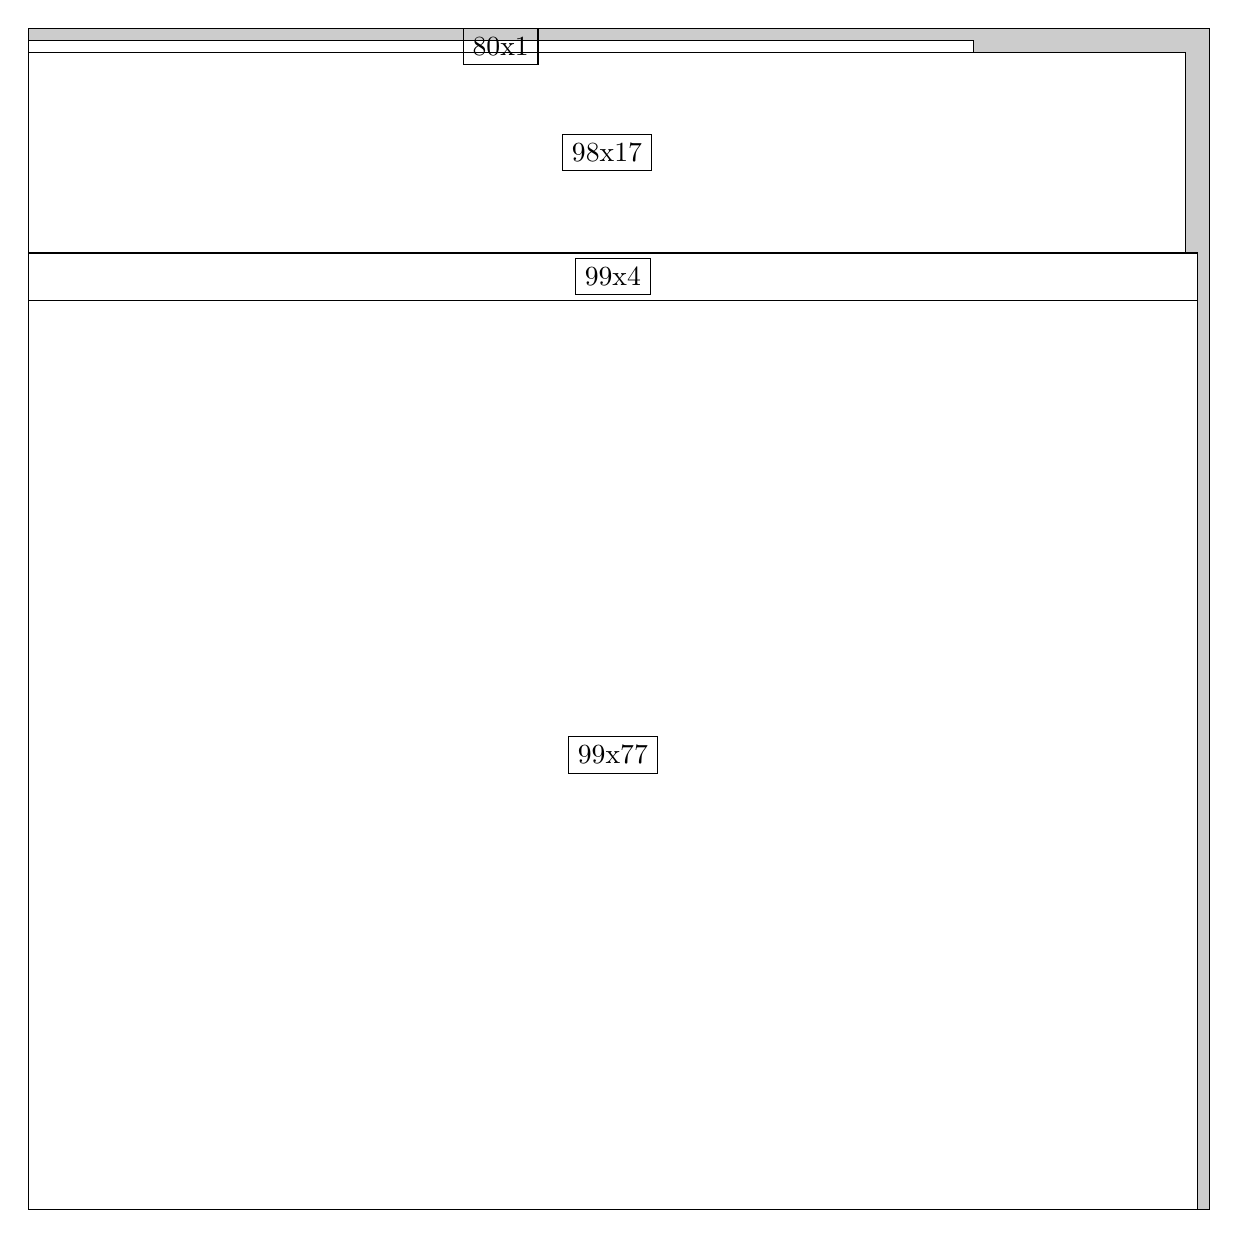
\begin{tikzpicture}[shorten >=1pt,scale=1.0,every node/.style={scale=1.0},->]
\tikzstyle{vertex}=[circle,fill=black!25,minimum size=14pt,inner sep=0pt]
\filldraw[fill=gray!40!white, draw=black] (0,0) rectangle (15.0,15.0);
\foreach \name/\x/\y/\w/\h in {98x17/0.0/12.15/14.7/2.55,99x77/0.0/0.0/14.85/11.549999999999999,99x4/0.0/11.549999999999999/14.85/0.6,80x1/0.0/14.7/12.0/0.15}
\filldraw[fill=white!40!white, draw=black] (\x,\y) rectangle node[draw] (\name) {\name} ++(\w,\h);
\end{tikzpicture}


w =98 , h =17 , x =0 , y =81 , v =1666
\par
w =99 , h =77 , x =0 , y =0 , v =7623
\par
w =99 , h =4 , x =0 , y =77 , v =396
\par
w =80 , h =1 , x =0 , y =98 , v =80
\par
\newpage


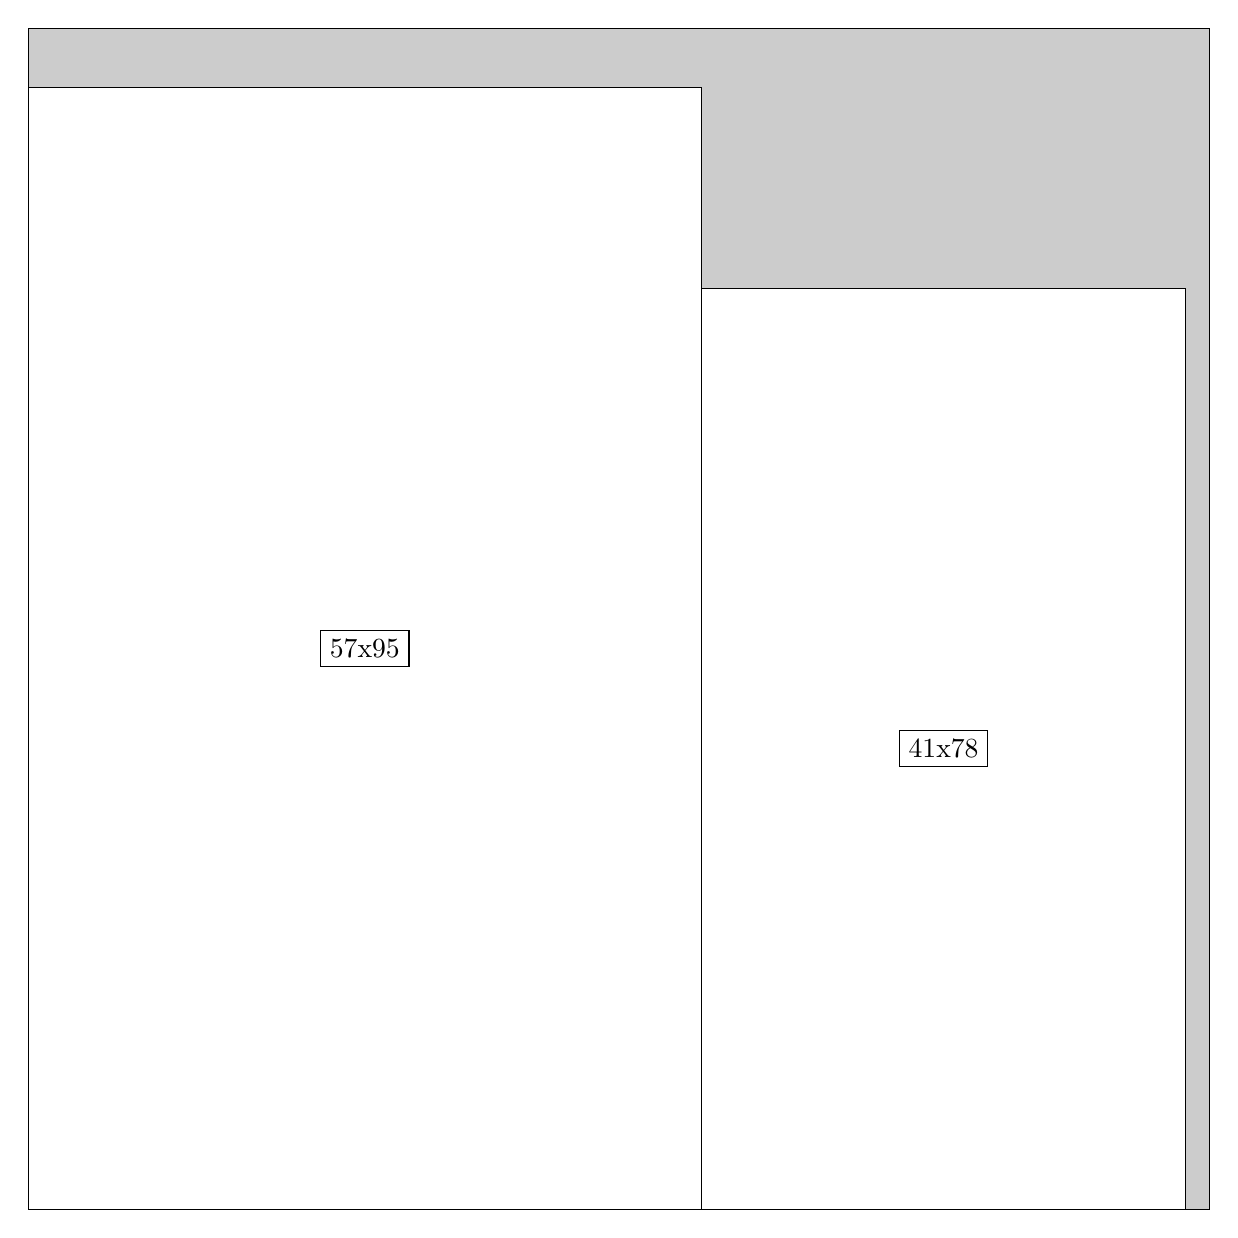
\begin{tikzpicture}[shorten >=1pt,scale=1.0,every node/.style={scale=1.0},->]
\tikzstyle{vertex}=[circle,fill=black!25,minimum size=14pt,inner sep=0pt]
\filldraw[fill=gray!40!white, draw=black] (0,0) rectangle (15.0,15.0);
\foreach \name/\x/\y/\w/\h in {57x95/0.0/0.0/8.549999999999999/14.25,41x78/8.549999999999999/0.0/6.1499999999999995/11.7}
\filldraw[fill=white!40!white, draw=black] (\x,\y) rectangle node[draw] (\name) {\name} ++(\w,\h);
\end{tikzpicture}


w =57 , h =95 , x =0 , y =0 , v =5415
\par
w =41 , h =78 , x =57 , y =0 , v =3198
\par
\newpage


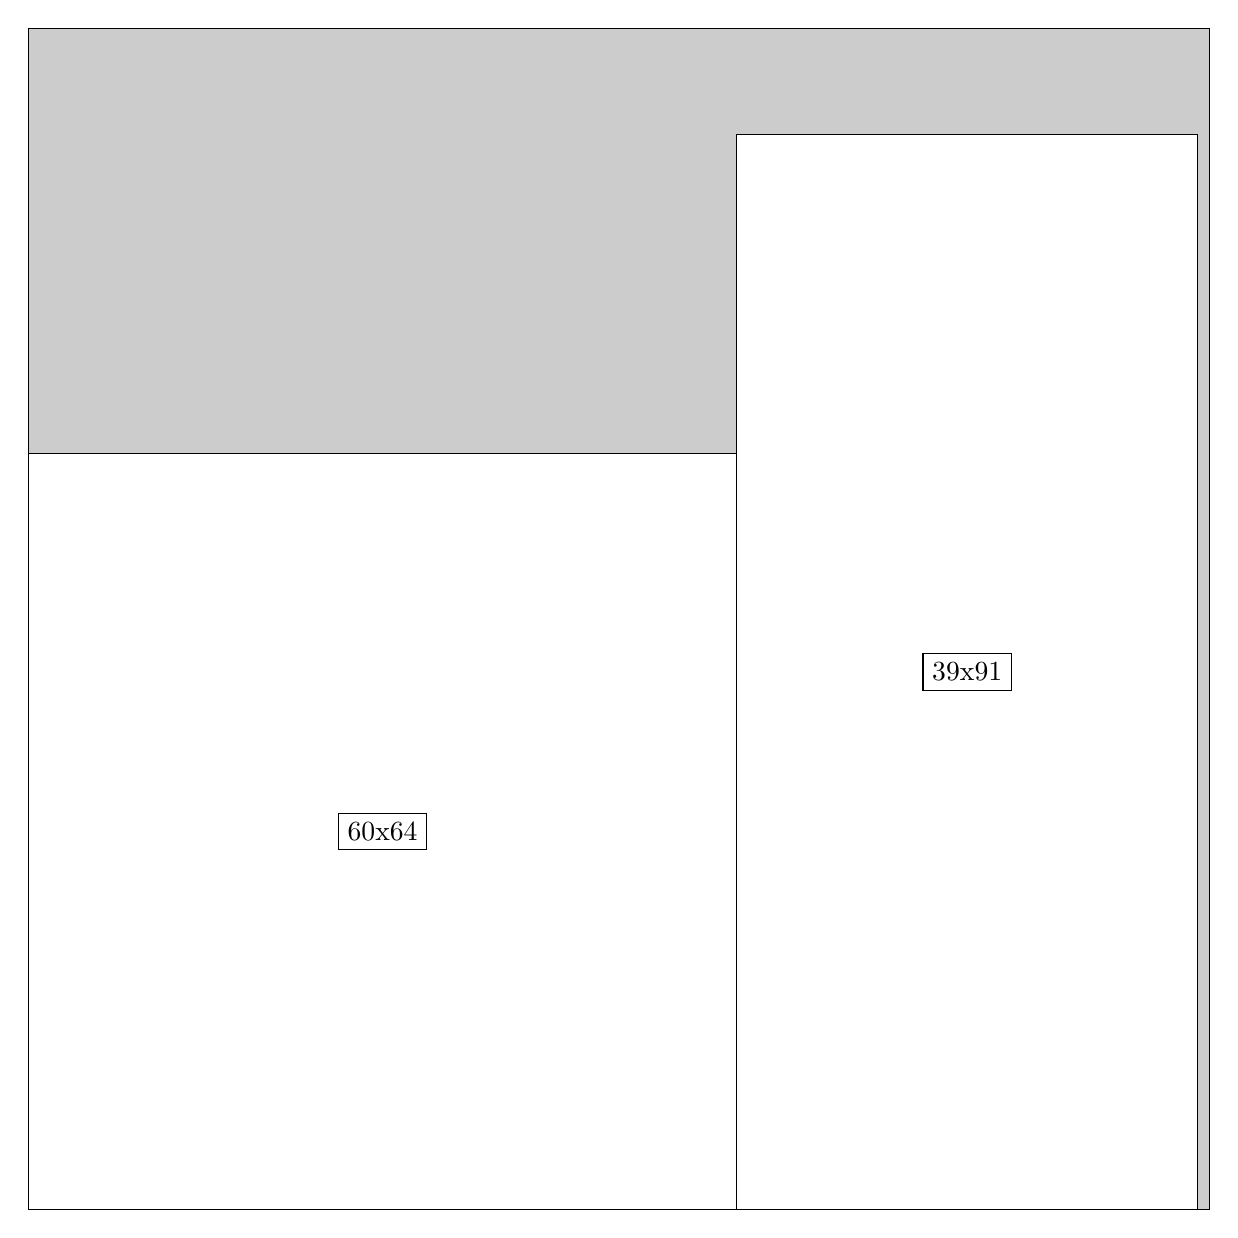
\begin{tikzpicture}[shorten >=1pt,scale=1.0,every node/.style={scale=1.0},->]
\tikzstyle{vertex}=[circle,fill=black!25,minimum size=14pt,inner sep=0pt]
\filldraw[fill=gray!40!white, draw=black] (0,0) rectangle (15.0,15.0);
\foreach \name/\x/\y/\w/\h in {60x64/0.0/0.0/9.0/9.6,39x91/9.0/0.0/5.85/13.65}
\filldraw[fill=white!40!white, draw=black] (\x,\y) rectangle node[draw] (\name) {\name} ++(\w,\h);
\end{tikzpicture}


w =60 , h =64 , x =0 , y =0 , v =3840
\par
w =39 , h =91 , x =60 , y =0 , v =3549
\par
\newpage


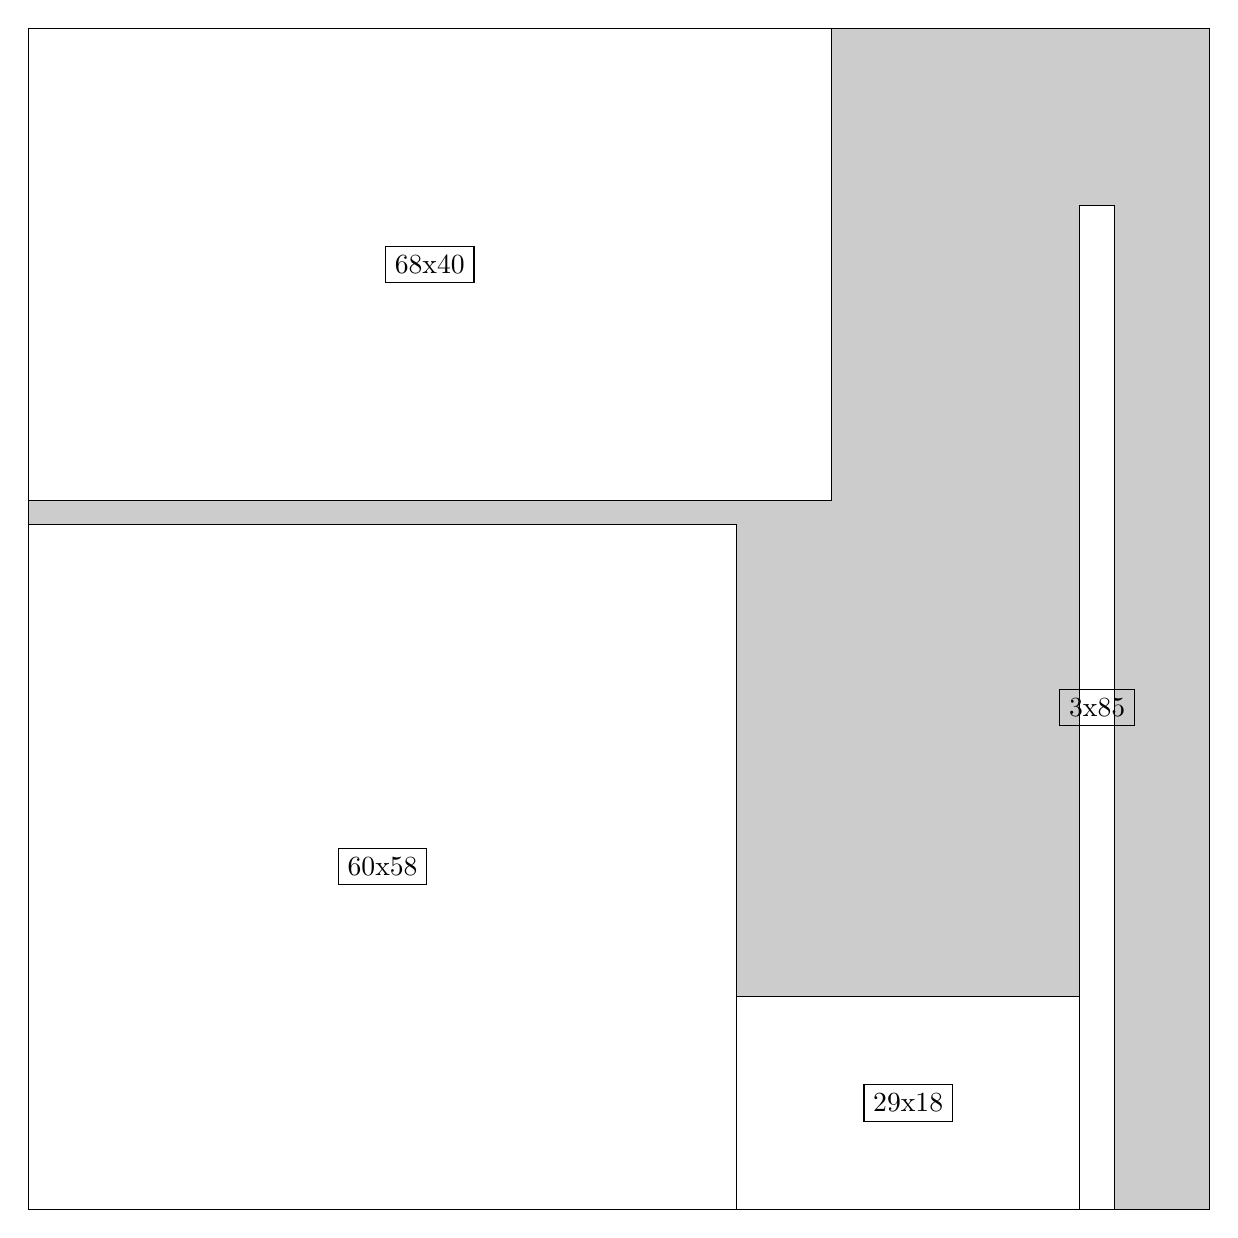
\begin{tikzpicture}[shorten >=1pt,scale=1.0,every node/.style={scale=1.0},->]
\tikzstyle{vertex}=[circle,fill=black!25,minimum size=14pt,inner sep=0pt]
\filldraw[fill=gray!40!white, draw=black] (0,0) rectangle (15.0,15.0);
\foreach \name/\x/\y/\w/\h in {60x58/0.0/0.0/9.0/8.7,68x40/0.0/9.0/10.2/6.0,29x18/9.0/0.0/4.35/2.6999999999999997,3x85/13.35/0.0/0.44999999999999996/12.75}
\filldraw[fill=white!40!white, draw=black] (\x,\y) rectangle node[draw] (\name) {\name} ++(\w,\h);
\end{tikzpicture}


w =60 , h =58 , x =0 , y =0 , v =3480
\par
w =68 , h =40 , x =0 , y =60 , v =2720
\par
w =29 , h =18 , x =60 , y =0 , v =522
\par
w =3 , h =85 , x =89 , y =0 , v =255
\par
\newpage


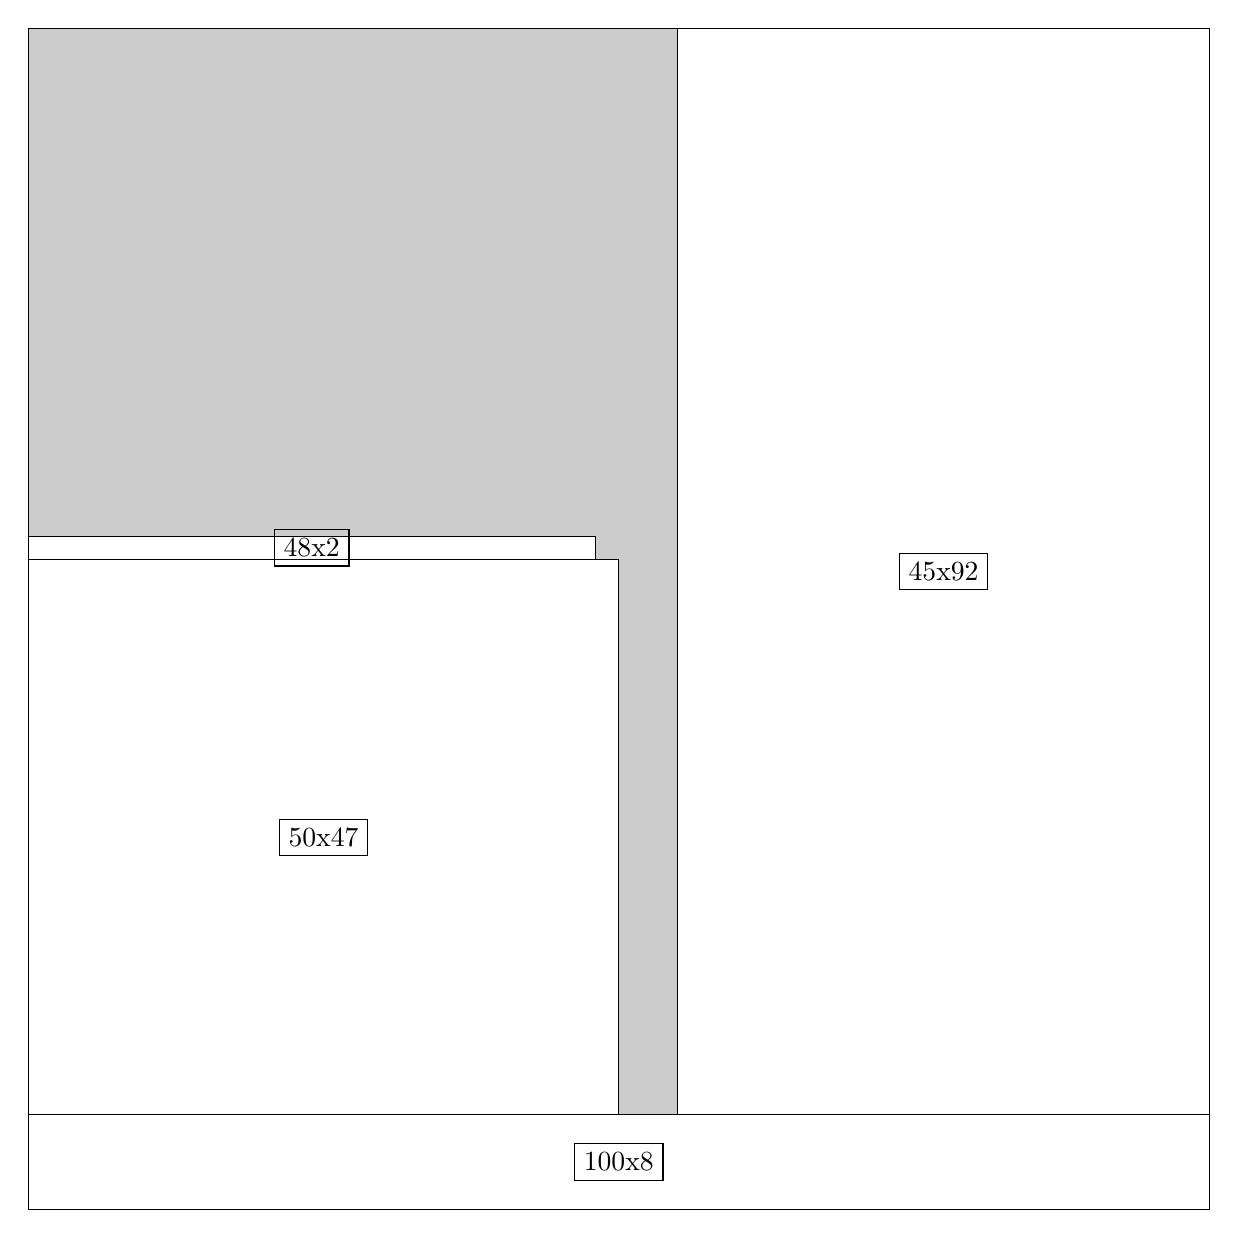
\begin{tikzpicture}[shorten >=1pt,scale=1.0,every node/.style={scale=1.0},->]
\tikzstyle{vertex}=[circle,fill=black!25,minimum size=14pt,inner sep=0pt]
\filldraw[fill=gray!40!white, draw=black] (0,0) rectangle (15.0,15.0);
\foreach \name/\x/\y/\w/\h in {45x92/8.25/1.2/6.75/13.799999999999999,50x47/0.0/1.2/7.5/7.05,100x8/0.0/0.0/15.0/1.2,48x2/0.0/8.25/7.199999999999999/0.3}
\filldraw[fill=white!40!white, draw=black] (\x,\y) rectangle node[draw] (\name) {\name} ++(\w,\h);
\end{tikzpicture}


w =45 , h =92 , x =55 , y =8 , v =4140
\par
w =50 , h =47 , x =0 , y =8 , v =2350
\par
w =100 , h =8 , x =0 , y =0 , v =800
\par
w =48 , h =2 , x =0 , y =55 , v =96
\par
\newpage


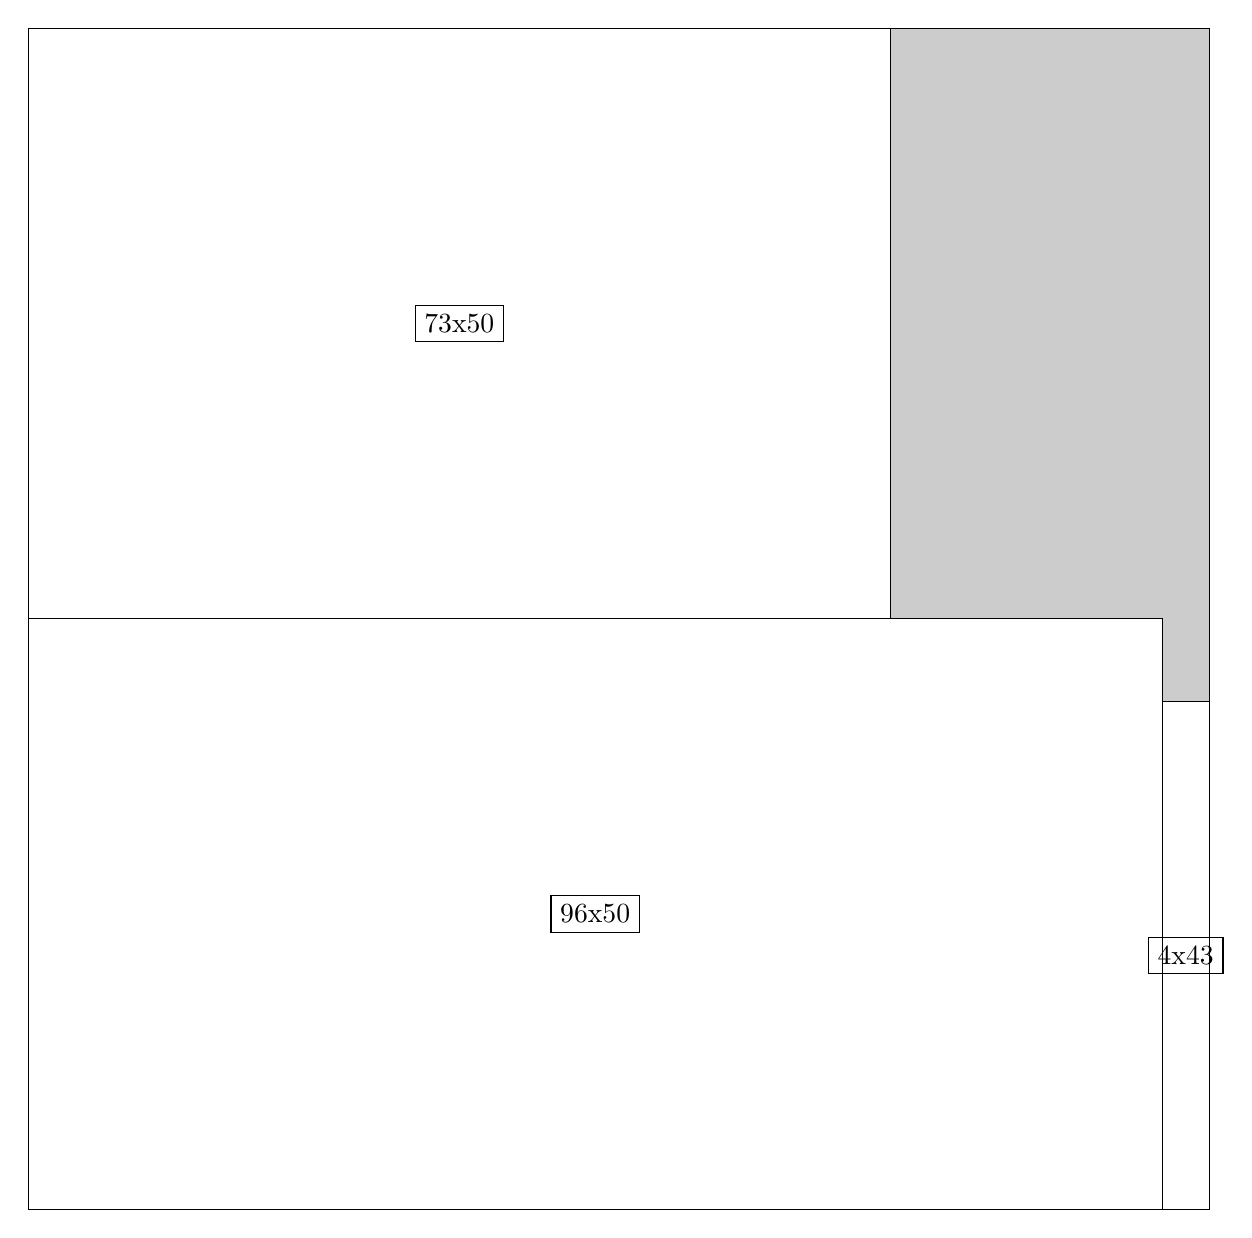
\begin{tikzpicture}[shorten >=1pt,scale=1.0,every node/.style={scale=1.0},->]
\tikzstyle{vertex}=[circle,fill=black!25,minimum size=14pt,inner sep=0pt]
\filldraw[fill=gray!40!white, draw=black] (0,0) rectangle (15.0,15.0);
\foreach \name/\x/\y/\w/\h in {96x50/0.0/0.0/14.399999999999999/7.5,73x50/0.0/7.5/10.95/7.5,4x43/14.399999999999999/0.0/0.6/6.45}
\filldraw[fill=white!40!white, draw=black] (\x,\y) rectangle node[draw] (\name) {\name} ++(\w,\h);
\end{tikzpicture}


w =96 , h =50 , x =0 , y =0 , v =4800
\par
w =73 , h =50 , x =0 , y =50 , v =3650
\par
w =4 , h =43 , x =96 , y =0 , v =172
\par
\newpage


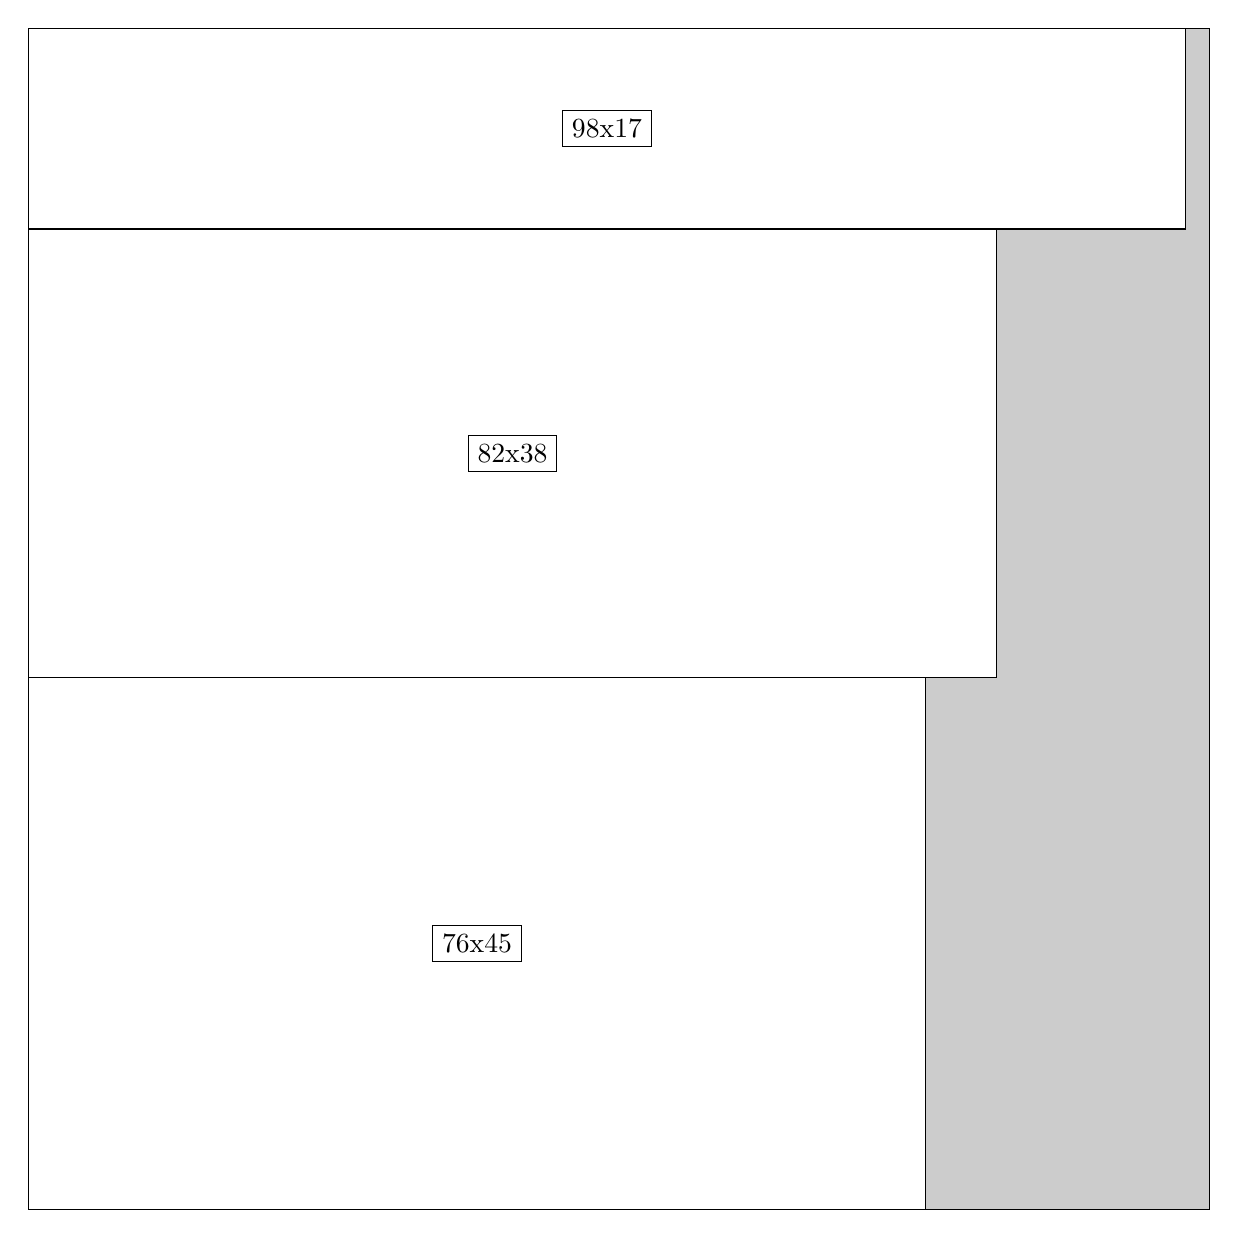
\begin{tikzpicture}[shorten >=1pt,scale=1.0,every node/.style={scale=1.0},->]
\tikzstyle{vertex}=[circle,fill=black!25,minimum size=14pt,inner sep=0pt]
\filldraw[fill=gray!40!white, draw=black] (0,0) rectangle (15.0,15.0);
\foreach \name/\x/\y/\w/\h in {76x45/0.0/0.0/11.4/6.75,82x38/0.0/6.75/12.299999999999999/5.7,98x17/0.0/12.45/14.7/2.55}
\filldraw[fill=white!40!white, draw=black] (\x,\y) rectangle node[draw] (\name) {\name} ++(\w,\h);
\end{tikzpicture}


w =76 , h =45 , x =0 , y =0 , v =3420
\par
w =82 , h =38 , x =0 , y =45 , v =3116
\par
w =98 , h =17 , x =0 , y =83 , v =1666
\par
\newpage


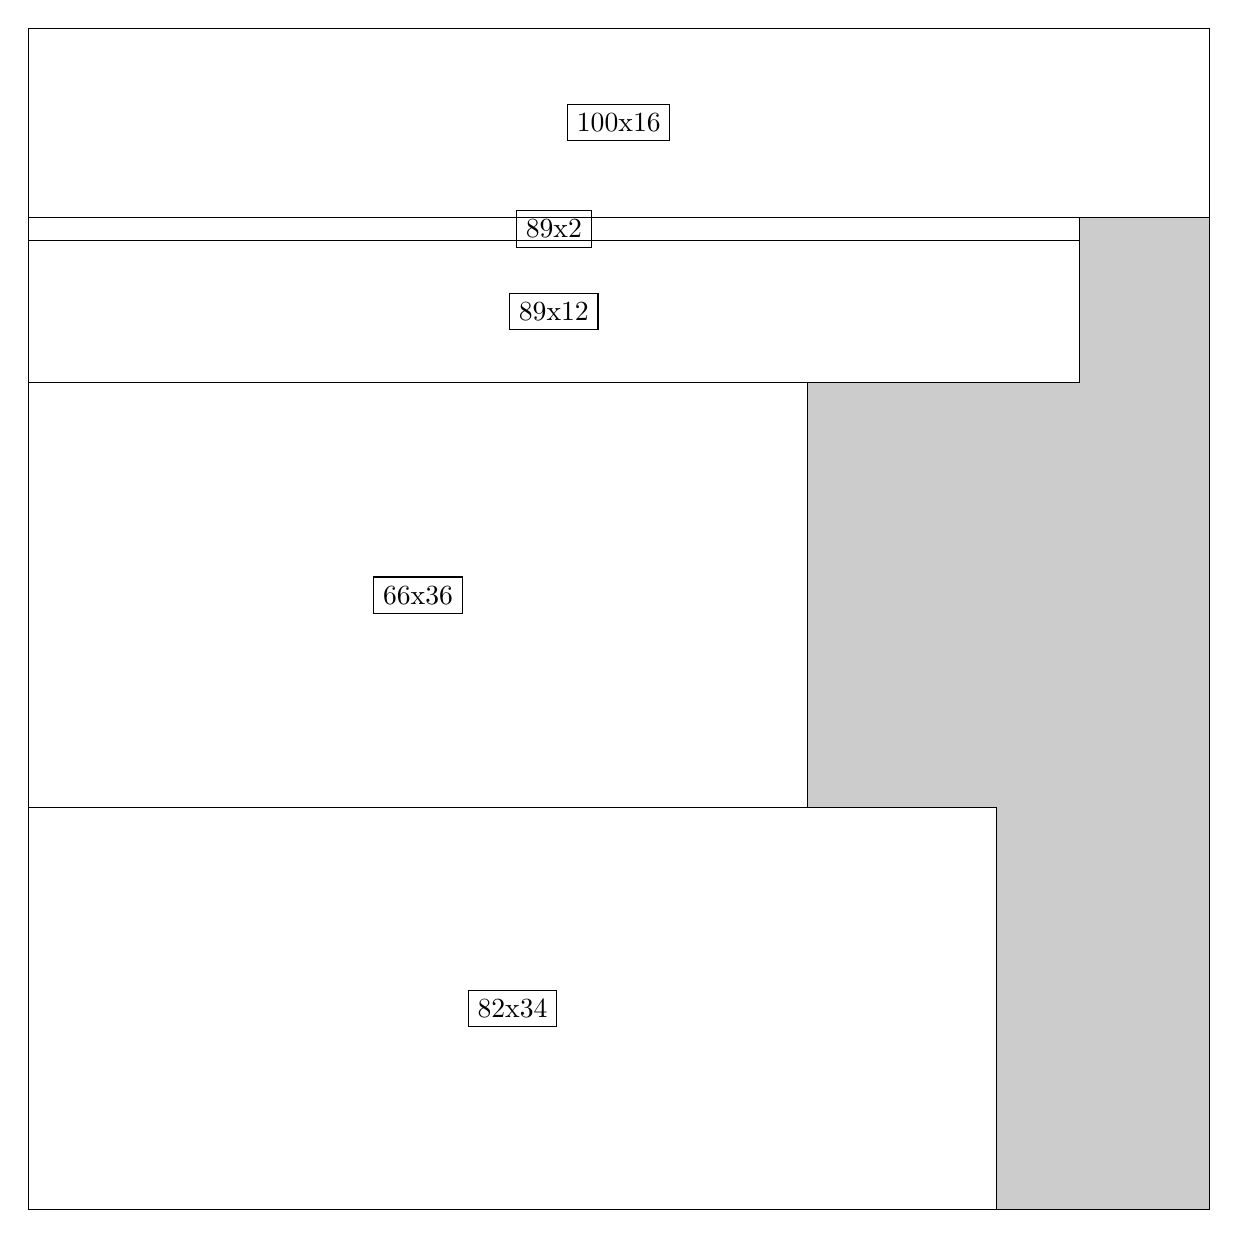
\begin{tikzpicture}[shorten >=1pt,scale=1.0,every node/.style={scale=1.0},->]
\tikzstyle{vertex}=[circle,fill=black!25,minimum size=14pt,inner sep=0pt]
\filldraw[fill=gray!40!white, draw=black] (0,0) rectangle (15.0,15.0);
\foreach \name/\x/\y/\w/\h in {82x34/0.0/0.0/12.299999999999999/5.1,66x36/0.0/5.1/9.9/5.3999999999999995,100x16/0.0/12.6/15.0/2.4,89x12/0.0/10.5/13.35/1.7999999999999998,89x2/0.0/12.299999999999999/13.35/0.3}
\filldraw[fill=white!40!white, draw=black] (\x,\y) rectangle node[draw] (\name) {\name} ++(\w,\h);
\end{tikzpicture}


w =82 , h =34 , x =0 , y =0 , v =2788
\par
w =66 , h =36 , x =0 , y =34 , v =2376
\par
w =100 , h =16 , x =0 , y =84 , v =1600
\par
w =89 , h =12 , x =0 , y =70 , v =1068
\par
w =89 , h =2 , x =0 , y =82 , v =178
\par
\newpage


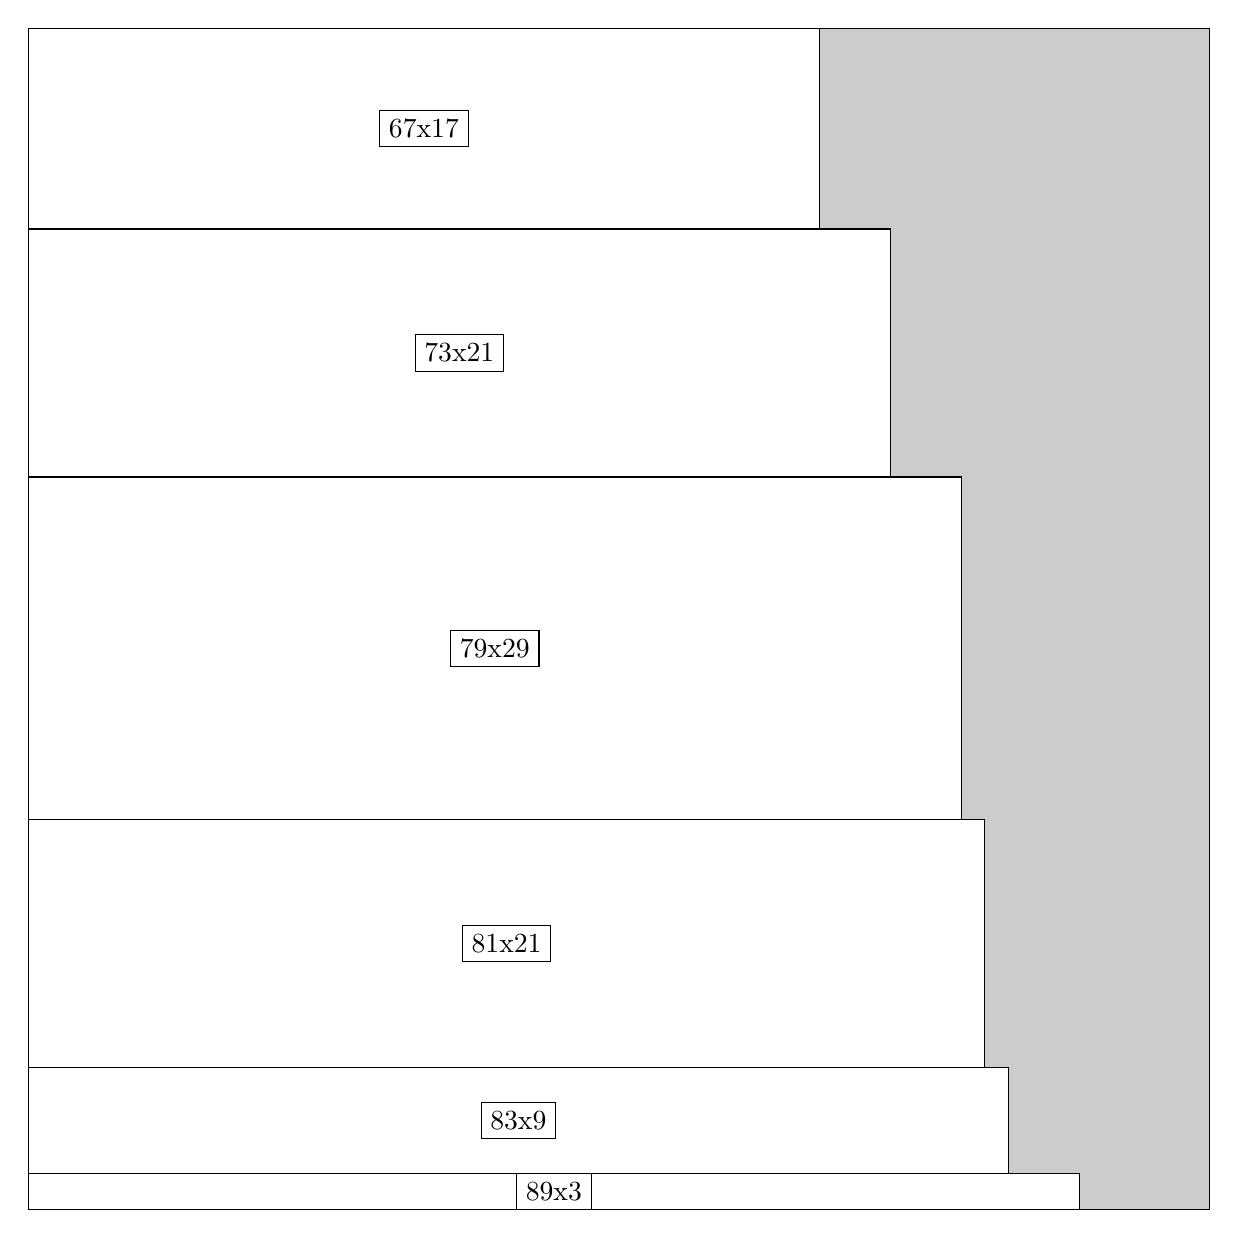
\begin{tikzpicture}[shorten >=1pt,scale=1.0,every node/.style={scale=1.0},->]
\tikzstyle{vertex}=[circle,fill=black!25,minimum size=14pt,inner sep=0pt]
\filldraw[fill=gray!40!white, draw=black] (0,0) rectangle (15.0,15.0);
\foreach \name/\x/\y/\w/\h in {83x9/0.0/0.44999999999999996/12.45/1.3499999999999999,79x29/0.0/4.95/11.85/4.35,81x21/0.0/1.7999999999999998/12.15/3.15,73x21/0.0/9.299999999999999/10.95/3.15,67x17/0.0/12.45/10.049999999999999/2.55,89x3/0.0/0.0/13.35/0.44999999999999996}
\filldraw[fill=white!40!white, draw=black] (\x,\y) rectangle node[draw] (\name) {\name} ++(\w,\h);
\end{tikzpicture}


w =83 , h =9 , x =0 , y =3 , v =747
\par
w =79 , h =29 , x =0 , y =33 , v =2291
\par
w =81 , h =21 , x =0 , y =12 , v =1701
\par
w =73 , h =21 , x =0 , y =62 , v =1533
\par
w =67 , h =17 , x =0 , y =83 , v =1139
\par
w =89 , h =3 , x =0 , y =0 , v =267
\par
\newpage


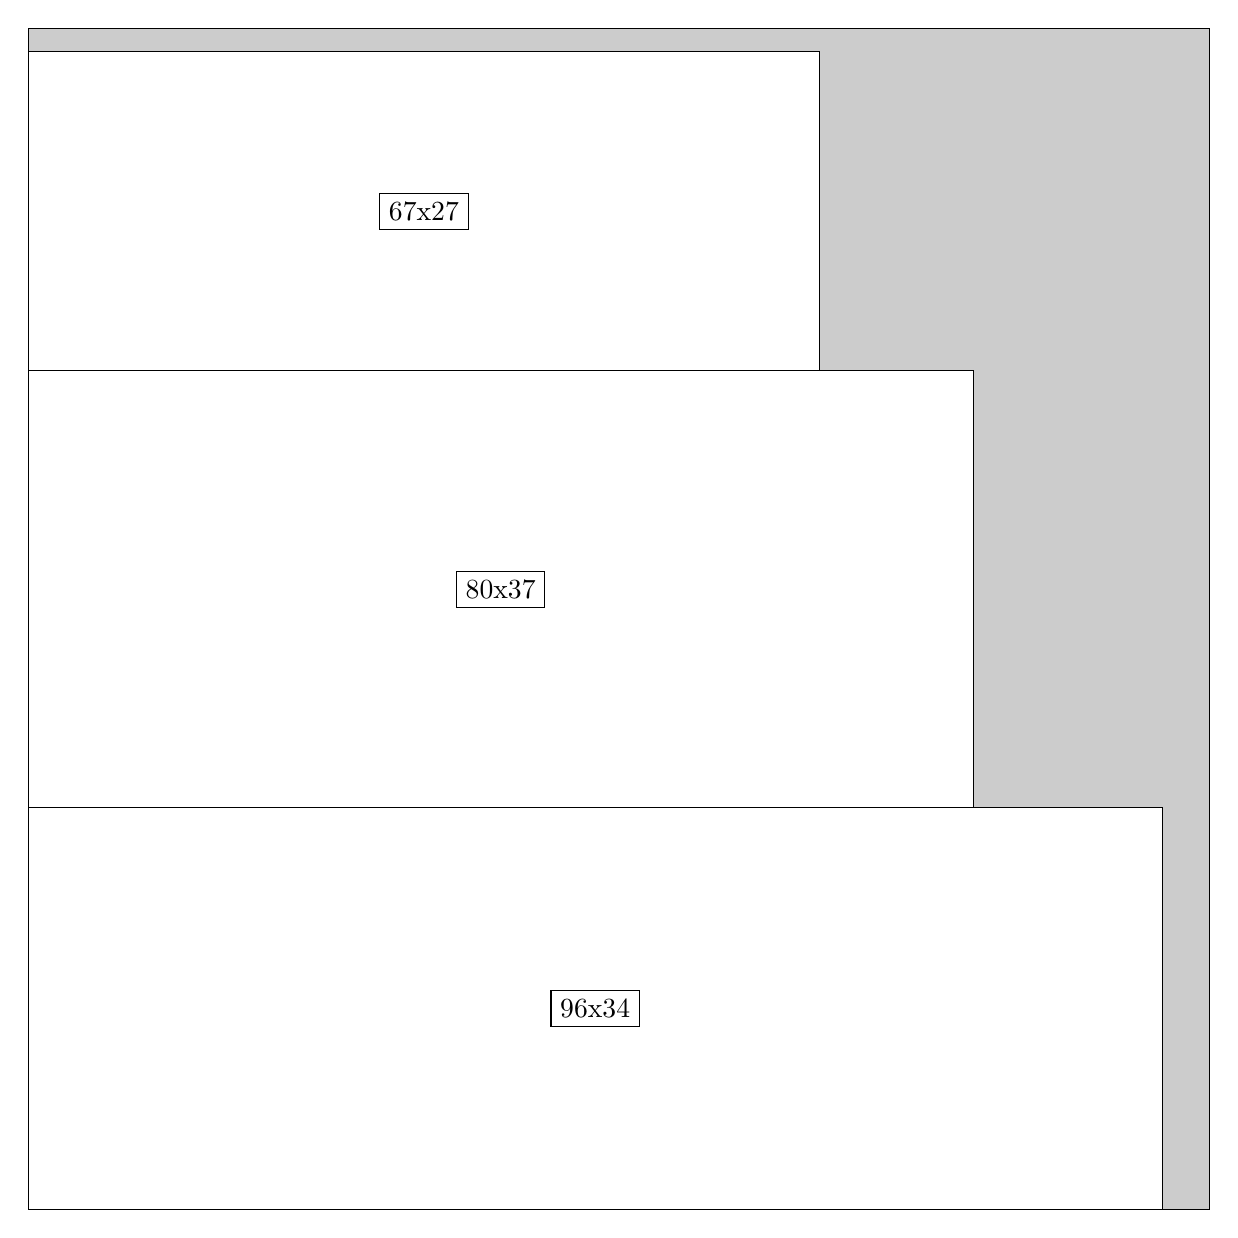
\begin{tikzpicture}[shorten >=1pt,scale=1.0,every node/.style={scale=1.0},->]
\tikzstyle{vertex}=[circle,fill=black!25,minimum size=14pt,inner sep=0pt]
\filldraw[fill=gray!40!white, draw=black] (0,0) rectangle (15.0,15.0);
\foreach \name/\x/\y/\w/\h in {96x34/0.0/0.0/14.399999999999999/5.1,80x37/0.0/5.1/12.0/5.55,67x27/0.0/10.65/10.049999999999999/4.05}
\filldraw[fill=white!40!white, draw=black] (\x,\y) rectangle node[draw] (\name) {\name} ++(\w,\h);
\end{tikzpicture}


w =96 , h =34 , x =0 , y =0 , v =3264
\par
w =80 , h =37 , x =0 , y =34 , v =2960
\par
w =67 , h =27 , x =0 , y =71 , v =1809
\par
\newpage


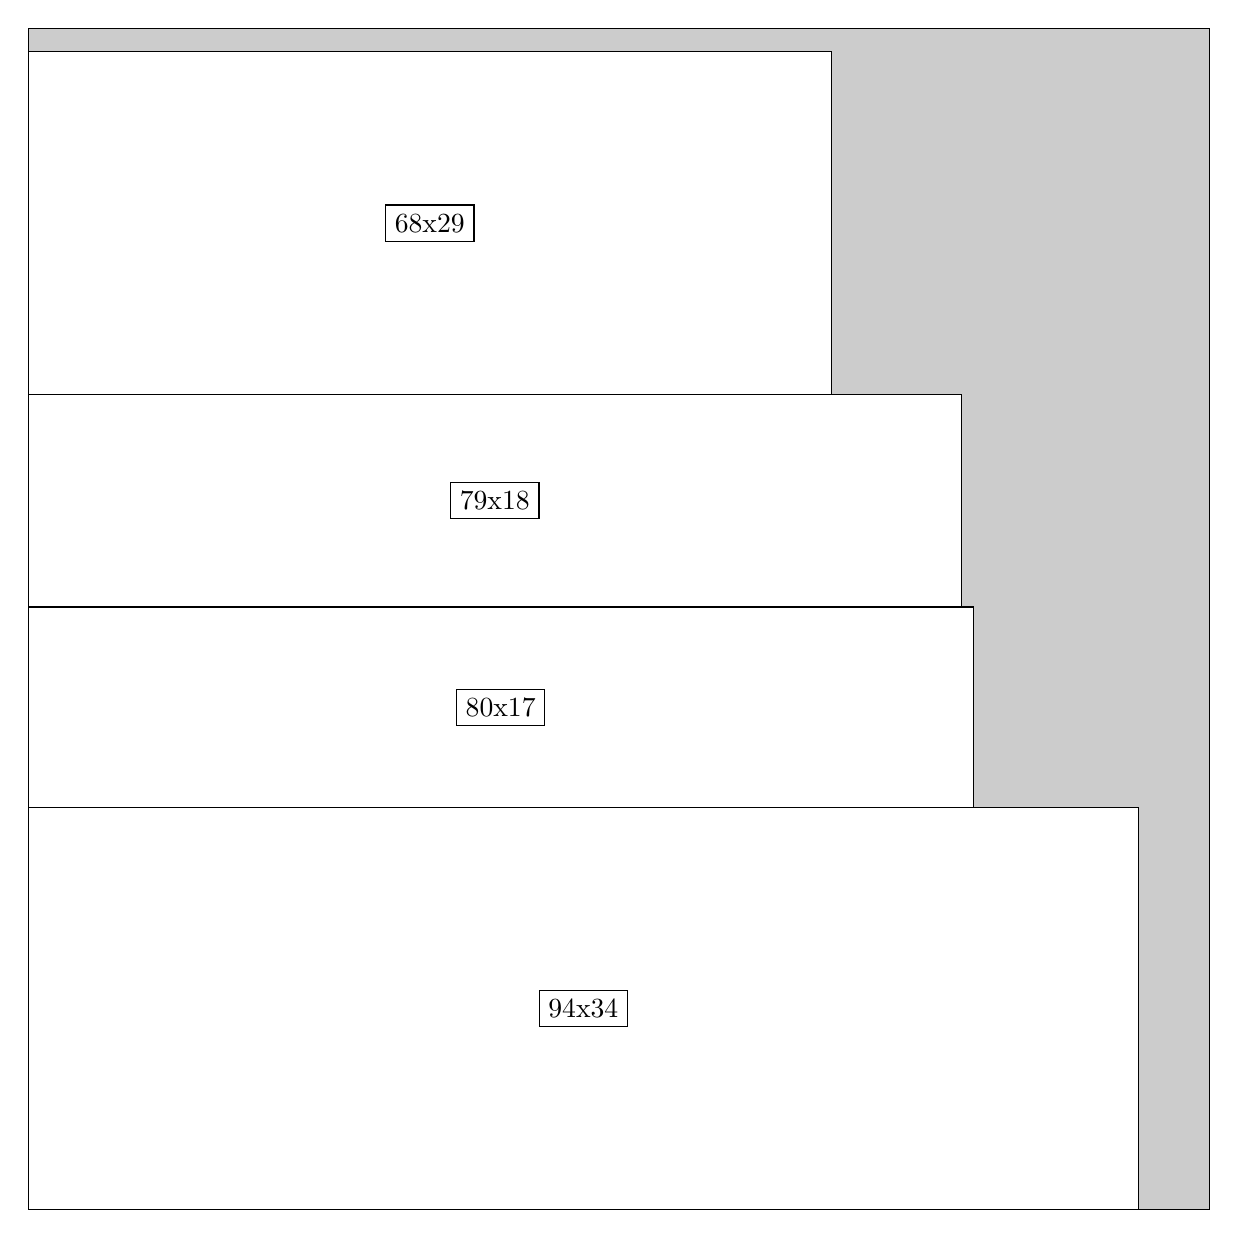
\begin{tikzpicture}[shorten >=1pt,scale=1.0,every node/.style={scale=1.0},->]
\tikzstyle{vertex}=[circle,fill=black!25,minimum size=14pt,inner sep=0pt]
\filldraw[fill=gray!40!white, draw=black] (0,0) rectangle (15.0,15.0);
\foreach \name/\x/\y/\w/\h in {94x34/0.0/0.0/14.1/5.1,68x29/0.0/10.35/10.2/4.35,79x18/0.0/7.6499999999999995/11.85/2.6999999999999997,80x17/0.0/5.1/12.0/2.55}
\filldraw[fill=white!40!white, draw=black] (\x,\y) rectangle node[draw] (\name) {\name} ++(\w,\h);
\end{tikzpicture}


w =94 , h =34 , x =0 , y =0 , v =3196
\par
w =68 , h =29 , x =0 , y =69 , v =1972
\par
w =79 , h =18 , x =0 , y =51 , v =1422
\par
w =80 , h =17 , x =0 , y =34 , v =1360
\par
\newpage


\end{document}